\documentclass[12pt]{article}
\usepackage{amsmath}
\usepackage{amssymb}
\usepackage{graphicx}
\usepackage{hyperref}
\usepackage{multicol}
\usepackage[latin1]{inputenc}
\usepackage{listings}
\usepackage{scrextend}

\usepackage{subcaption}

\title{ComS 342\\Recitation 2, 10:00 Tuesday\\Homework 2}
\author{Sean Gordon}
%\date{09/09/2019}

\begin{document}
\maketitle


%\begin{addmargin}[2.5em]{1.5em}
\noindent 1) $(+ (* 10\ 2) 1)$ and $(- (* 9\ 3) 6)$

\noindent 2)


\begin{figure}[h!]
  \centering
  \begin{subfigure}[b]{0.4\linewidth}
    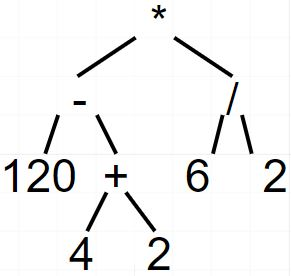
\includegraphics[width=\linewidth]{ComS342_HW2_2a.jpg}
    \caption{(* (- 120 (+ 4 2)) (/ 6 2))}
  \end{subfigure}
  \begin{subfigure}[b]{0.4\linewidth}
    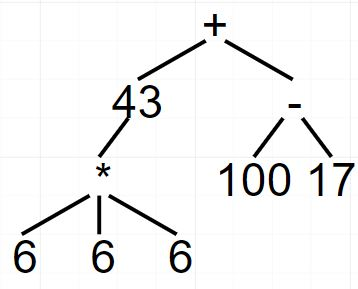
\includegraphics[width=\linewidth]{ComS342_HW2_2b.jpg}
    \caption{(+ 43 (* 6 6 6) (- 100 17))}
  \end{subfigure}
  \label{fig:Pt2}
\end{figure}





\noindent 3a) AST provides functions and helpers to work with the program, while Evaluator makes use of those functions to compute the result of the program. \\

\noindent b) Using pattern $(+ (* 10\ 2) 1)$, 

%\end{addmargin}
\end{document}